%%%%%%%%%%%%%%%%%%%%%%%%%%%%%%%%%%%%%%%%%%%%%%%%%%%%%%%%%%%%%%%%%%%%%%%%%%%%%
\chapter{Implementation of Identity Management}\label{chap:implementation}
%%%%%%%%%%%%%%%%%%%%%%%%%%%%%%%%%%%%%%%%%%%%%%%%%%%%%%%%%%%%%%%%%%%%%%%%%%%%%
\chapterstart

 Based on this risk assessment a small solution representing the identity management is implemented. The procedure of conducting a risk assessment should help developers to choose appropriate authentication and authorization methods for a particular use case. The chapter is split up into two parts. The first part describes how the architecture of the solution was chosen and the second part explains how the identity management of the solution works. 


\section{Architecture}
\label{architecture}

The Sakimura et al. (2014) explains that modern applications have different requirements than their predecessors, due to new distributed architectures that allow enterprises to be more flexible. Cloud or microservice architectures require different interactions between applications.The below (figure~\ref{fig:architecture-identityserver}) shows the most common interactions for modern applications [cf. (\cite{Sakimura:2014:OpenIDConnect})].

\begin{figure}[h]
	\centering
	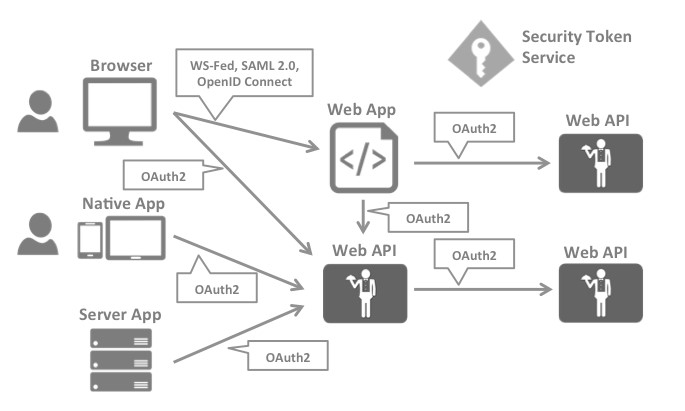
\includegraphics[width=0.9\linewidth]{images/architecture-identityserver}
	\caption[Architecture IdentityServer4]{Architecture IdentityServer4 (\cite{Brock:2018:ID4}}
	\caption{Architecture IdentityServer4 (\cite{Brock:2018:ID4})}
	\label{fig:architecture-identityserver}
\end{figure}

For example, a browser might call a Web App, and a Web App calls a Web API or perhaps a Native App calls a Web API, which is calling another Web API. Each application has to implement security functions to maintain a secure flow throughout these interactions. Implementing this security features for each involved application leads to a lot of duplicated code and inconsistencies. A different approach to implement security throughout these flows is using a token service. A token service brings the benefit of being able to encapsulate these security functions. Security functions can be updated and hosted at a single point which prevents duplicated functions across applications and security flaws. The advantages of a token service or token based application are also outlined in the section \ref{tokenBasedAuthentication}. Furthermore the chapter \ref{tokenBasedAuthentication} hold examples of JSON Tokens and how they are asserted. The concept of JSON Tokens is very important in token-based authentication systems and ensures confidentiality and integrity [cf. (\cite{Sakimura:2014:OpenIDConnect})].

Based on the chapter \ref{riskassessment} the architecture of the authentication system for the use case described in chapter \ref{usecase} is chosen. The LOA for identity proofing should be two, according to the risk assessment. Other LOA for identity proofing are covered in chapter \ref{identityProofing}. The second level of assurance for identity proofing suggests that no real-world existence of the claimed identity has to be present. The presentation of the real-existence can be either remote or physical. This means for our example that the user does not have to be physical present, which would be the case for passport controls. The users can sufficiently prove their identity remotely. Additionally to the LOA figure~\ref{fig:ialflow} suggest, in consideration of a unique resolvent of an identity, that accepting references is ok. This means that not always a full presentation of an identity is needed, for this use case claims are acceptable. Therefore a federation solution is recommended. The federation solution should furthermore offer Single-Sign on because of the requirements described in \ref{usecase}. The Single Sign-on solution uses OAuth and OpenID Connect in view of the facts that were pointed out in \ref{singlesignon}. To implement federation a token server is implemented. Since the first federation is used in this example also the the according federation assurance level based on the risk assessment is considered. It was evaluated to use the first level of assurance. The first level of assurance states to use a bearer assertion signed with approved cryptography by an IdP like OpenID Connect Basic Client profile. Therefor the solution will use an token service which login functionality is accepting one distinct authentication factor and asserts the user with bearer tokens. In order to receive a token form the token server a users have to successfully proof their identity. In order to prove their identity the users have to provide valid credentials to authenticate at the service. The authentication assurance level analyzed in the chapter \ref{riskassessment} helps to chose the factors for the solution. According to this initial risk assessment the level of assurance should be two. Other LOA are described in chapter \ref{authentication}. The second level of authentication assurance suggests to use at least two distinct authentication factors and the use of strong cryptographic techniques. However, the first level for authentication will be used in this solution because two distinct authentication factors would normally just be used for really sensitive personal data like in a bank app. The first level of assurance for authentication suggest the use of one authentication factor. 

This leads to a simple modern architecture consisting of an Identity Server, a API and an Angular Application. The Identity Server is using bearer tokens and provides Single Sign-on. The API is just accessible with a validates a token. If a valid token is provided it sends back data. In this case the API application also serves as a resource server. And last but not least, a simple Angular App which provides a login functionality and a page that is just accessible with a valid token.


\section{Implementation}

The implementation is based on the architecture descibed in \ref{architecture}. The languages chosen for the example application are C\# and Angular 2. The solution is created with a very useful ASP.NET framework called Identity Server4. Identity Server4 uses the specifics of OpenID Connect and OAuth 2.0 to enable authentication and authorization related features. Features include authentication as a Service, which provides a centralized login logic for all applications, Single sign-on, Access Control for APIs and Federation Gateway. The Identity Server 4 will be used as a Token Server in the practical part [cf. (\cite{Brock:2018:ID4})]

The project illustrating the use of Identity Server and the benefits of OpenID Connect an OAuth is a Visual Studio Project mostly written in C\# and Typescript. The project example for Identity Server includes four different projects:

\begin{itemize}
	\item Identity Server - The Identity Server is a ASP.NET Core Project with basic implementation of an Identity Server which serves as a Token Server. 
	\item ProjectApiNetCore - This application is a ASP.NET Core 2.0 API Application with basic API that returns the users claims if he is authenticated.
	\item Angular Client - The Angular Client is a ASP.NET Core MVC Angular Project used as a client that can be accessed by an End-User who can authenticate with the Identity Server and requests protected resources of the API ProjectApiNetCore.This project uses the Implicit Code Flow. 
	\item MVC Client - The MVC Client is a ASP.NET Core MVC Project used as a Client that can be accessed by an End-User and can authenticate with the Identity Server and requests protected resources of the API ProjectApiNetCore. This project uses the Hybrid Code Flow. 
\end{itemize}



\paragraph{Identity Server}

This project is using the IdentityServer4 library by Brock Allen and Dominick Baier. The Project works as a Token Server which means that the Identity Server Project is responsible for the authentication of the user, managing the identities and provide and approve tokens. Furthermore, the Identity Server implements different Authentication Flows.


\begin{figure}[h]
	\centering
	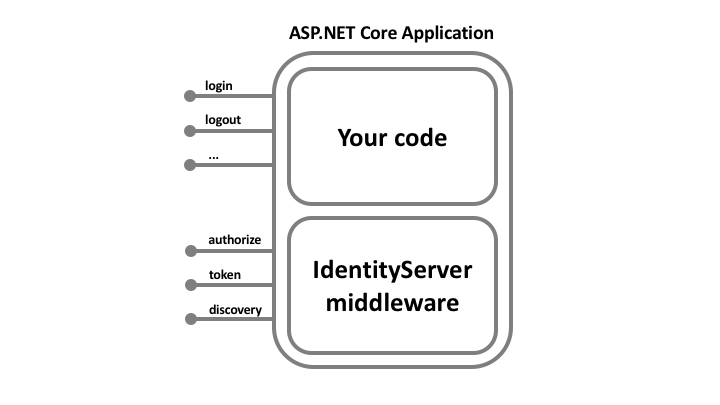
\includegraphics[width=0.6\linewidth]{images/middlewareIdentityServer}
	\caption{IdentityServer Middleware}
	\label{fig:middlewareidentityserver}
\end{figure}
 

IdentityServer4 adds endpoints of OAuth 2.0 and OpenID Connect to an arbitrary ASP.NET Core application as shown in figure~\ref{fig:middlewareidentityserver}. The identity server can be as complex as the developer wants but Brock \& Baier (2018) recommend to keep the attack surface as small as possible by just including authentication related UI only [cf. (\cite{Brock:2018:ID4})]. 


For the basic setup, the Identity Server has to be added to the StartUp class and to ensure a secure communication a certificate is created to sign the request. For the basic setup, Identity Server provides us with DeveloperSigningCredentials which provides a dummy certificate. In this example application, a real certificate is included. 

\begin{figure}[h]
	\centering
	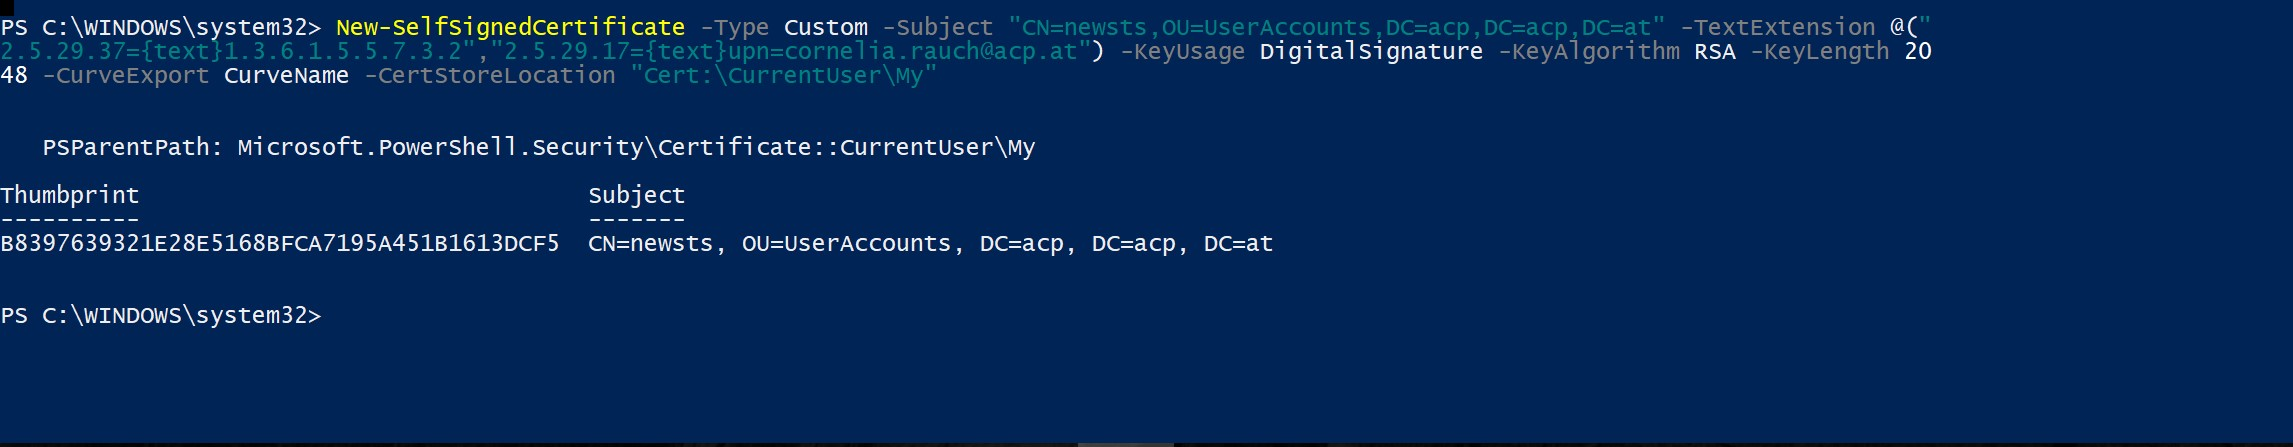
\includegraphics[width=0.9\linewidth]{images/self-signed-certicate}
	\caption{Self signed Certicate with Powershell}
	\label{fig:self-signed-certicate}
\end{figure}

The certificate used in this application was created with Powershell as shown in figure~\ref{fig:self-signed-certicate}. The algorithm used in this certificate is RSA. Depending on the algorithm that is used in the certificate a similar hashing algorithm has to be used for the Client Secret.


The API Resources include the available APIs that can be called and included in the scope of a request. The Identity Resources are Resources that can be included in the returning id\_token. The clients are the available clients that can be configured and can use the Identity Server. Those client Configurations indicate which Authorization Flow is used and how to retrieve id\_token, access\_token, and a possible refreh\_token. For simplifying reasons, Identity Server provides an in Memory User Storage which can be used for testing reasons. Other ways to define users are via .NET Core Identity or IdentityServer4 EntityFramework. For the purpose of this implementation this test users where included in the Identity Server application:
\begin{enumerate}
	\item User1:
	\begin{itemize}
		\item  Username: bob
		\item  Password: bob
	\end{itemize} 
	\item User2:
	\begin{itemize}
		\item  Username: alice
		\item  Password: alice
	\end{itemize} 
\end{enumerate}

After the basic setup of the Identity Server, it can be examined if the Identity Server is running correctly by calling the discovery document. The discovery document can be used by the Clients and APIs to retrieve necessary configuration data. The Identity Server has to run at local port 5000 and the navigation path for the browser is:
\url{http://localhost:5000/.well-known/openid-configuration}.

\begin{figure}[h]
	\centering
	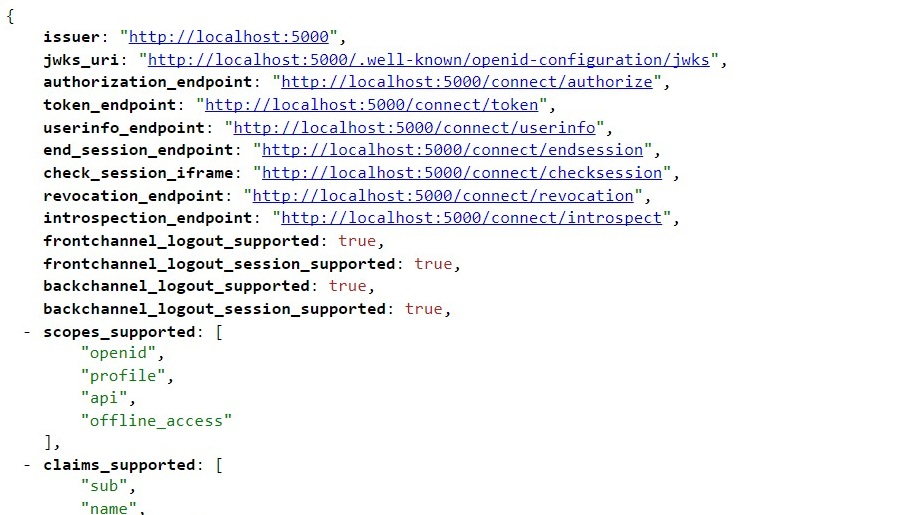
\includegraphics[width=0.8\linewidth]{images/openid-discovery-document}
	\caption{OpenID Discovery Document}
	\label{fig:openid-discovery-document}
\end{figure}
The discovery document shown in figure~\ref{fig:openid-discovery-document} is located at a well-known location and is containing key-value pairs as a JSON structure. The key-value pairs in the discovery document represent multiple endpoints that are used to authenticate a user including URIs of the authorization, token, userinfo, and public-keys endpoint. The use of a discovery document brings more flexibility to the protocol. The application should have the discovery URL hard-coded in the application according to (\cite{Google:2018:IdentityPlatform}) the discovery document URL can then be used to fetch endpoints from the document and use them to send an authentication request for example [cf. (\cite{Google:2018:IdentityPlatform})].

The metadata that is seen in \ref{fig:openid-discovery-document} is a mixture of required elements with some recommended ones that are implemented by the Identity Server. The required elements are issuer, authorization\_endpoint, token\_endpoint, jwks\_uri, response\_types\_supported, subject\_types\_supported and id\_token\_signing\_alg\_supported. The issuer, in this case, is this Identity Servers address. The authorization\_endpoint is the URL OAuth 2.0 Authorization Endpoint. The user is redirected to the authorization server's authorization endpoint for authentication and authorization. The authentication request that is sent to the authorization server can have different request parameters. These request parameters are defined by OAuth 2.0 and additional request parameters defined by OpenID Connect. The token\_endpoint is the URL of the OAuth 2.0 Token Endpoint. The RP can request access or optionally refresh tokens from the token endpoint. The user\_endpoint can be used to request additional information concerning the user. The response\_types\_supported is a important information about what kind of response is supported and ultimately what kind of authentication flow can be used based on that information described in chapter \ref{chap:authenticationandauthorization}. The subject\_types\_supported is a list of subject identifier types. Moreover, last but not least id\_token\_signing\_alg\_supported is used to find out which JWS is signing algorithm is used to encode the ID token and get the claims of the JWT. The algorithm RS256 must be included [cf. (\cite{Sakimura:OIDCC}, (\cite{Sakimura:OIDCD}))].. 

\begin{figure}[h]
	\centering
	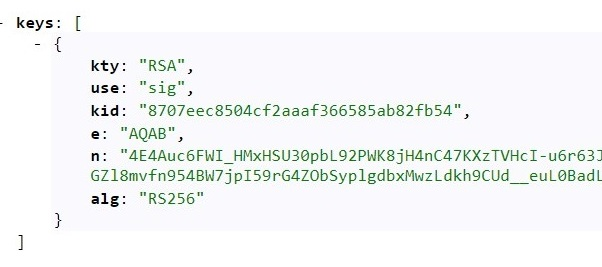
\includegraphics[width=0.7\linewidth]{images/jwkDiscovoryDocument}
	\caption{JWKS Endpint}
	\label{fig:jwkdiscovorydocument}
\end{figure}

The jwks\_endpoint is worth a closer look. JWKS SET is published to the JWKS endpoint. The keys shown in figure~\ref{fig:jwkdiscovorydocument} can be rolled over by periodically adding new keys to the JWK Set. This also indicates if the cryptographic algorithms are configured correctly. For example the message is using the kid of signing key in the JOSE Header to indicate which key has to be used to validate the signature. The algorithm used by the signing party has to be supported by the recipient and can be either an Asymmetric Signature or a Symmetric Signature. 
When using RSA or ECDSA signatures, the alg Header Parameter has to be set to the correct algorithm, and the private key used to sign must be associated with the public key published by the sender. When using MAC-based signatures, the alg Header Parameter has to be set to the correct algorithm, and the MAC key is the octets of the UTF-8 representation of the client\_secret. MAC-based signatures cannot be used by public Clients because they cannot keep secrets.  All metadata types are listed in the specification of OpenID Discovery Document from Sakimura et al. (2014) [cf. (\cite{Sakimura:OIDCD}))]. 

After calling the OpenID discovery document and the JWKS endpoint, one can be ensured that the basic setup of the IdentityServer works. After that a resource that is worth beeing protected by the Identity Server has to be created. 

\paragraph{ProjectApiNetCore}

This ProcjectApiNetcore is an ASP.NET Core application. This application represents the Resource Server and serves the Protected Resources. In this particular example, the API provides a list of Products the user bought from the company and the possibility to download the report that gives information about the current state of the product. The example API provides dummy data for the particular request. For easy testing of the API and designing the API, swagger.io is used. Furthermore, swagger.io (\url{https://swagger.io/}) gives a nice developer experience with an interactive API documentation. In addition, it is possible to generate code out of the swagger documentation for different programming languages with tools like NSwag (\url{https://github.com/RSuter/NSwag}).

\begin{figure}[h]
	\centering
	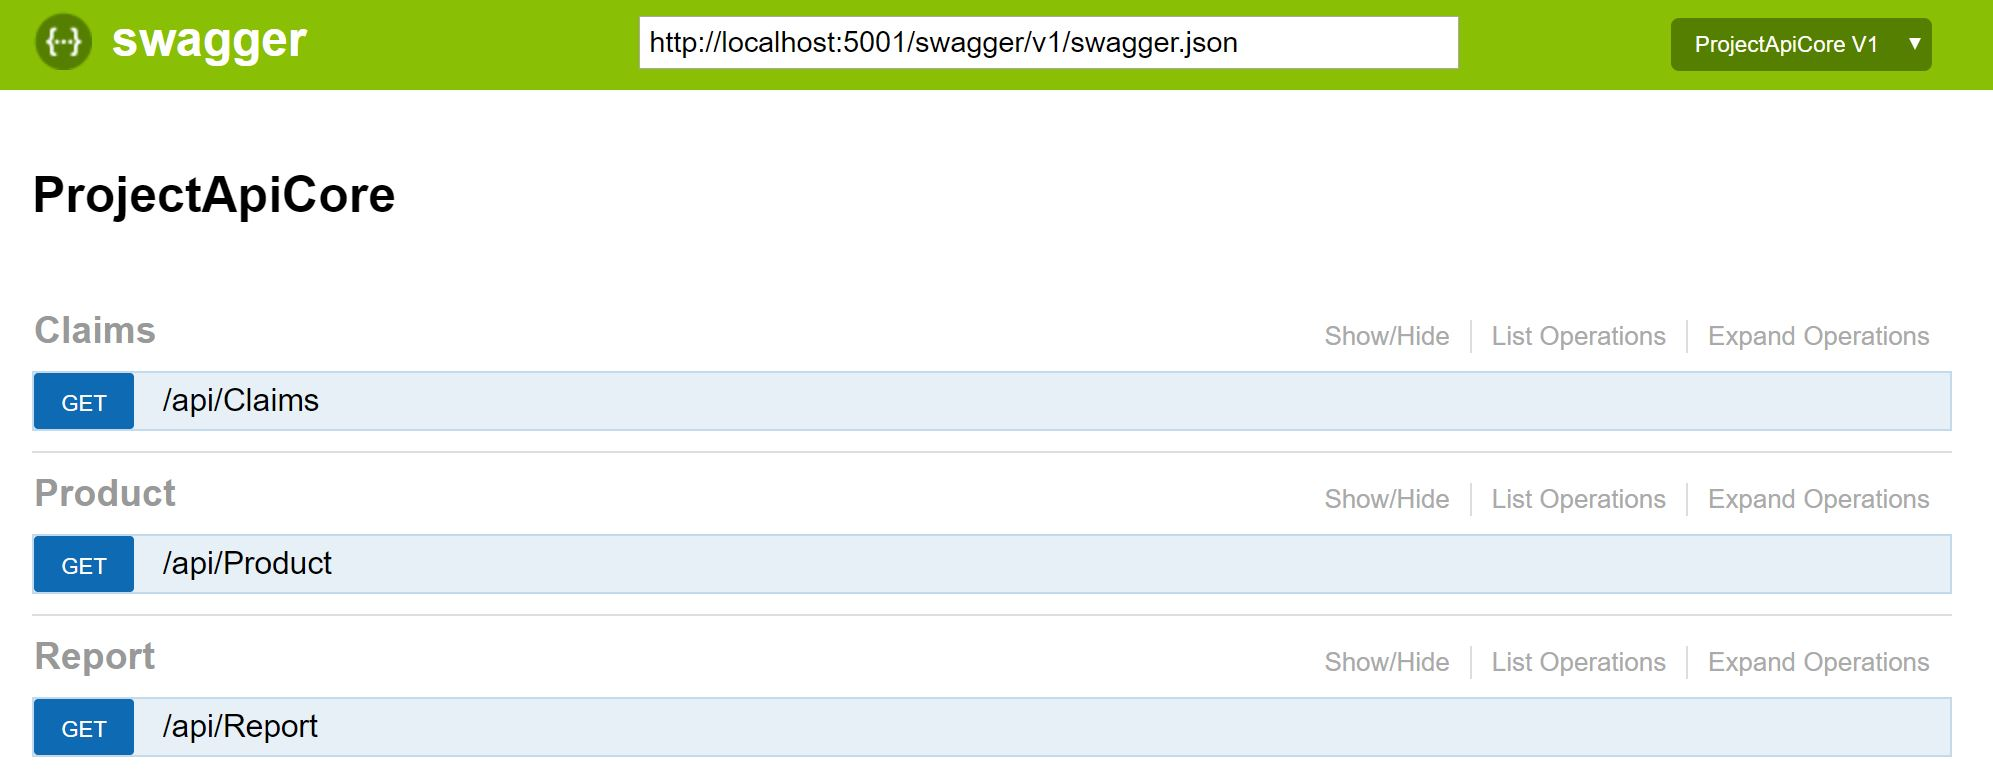
\includegraphics[width=0.7\linewidth]{images/apis}
	\caption{API documentation with Swagger}
	\label{fig:apis}
\end{figure}

All of the routes shown in figure~\ref{fig:apis}, are secured with the help of the IdentityServer4.AccessTokenValidation NuGet package. Each Controller gets an Authorize annotation. 
To configure the right authentication method, ASP.NET Core 2.0 offers the possibility to add the authentication to the pipeline with Dependency Injection via the method Configure Services in the Startup.class.
In the StartUp class of the API Project the AddAuthentication with the Value "JwtBearerDefaults.AuthenticationScheme" makes "Bearer" the default authentication scheme. With the AddIdentityServerAuthentication it is defined which Token server can be used to validate the incoming token and make sure that this token is from a trusted issuer. It adds the Identity Server access token validation handler into DI and also it is checked if the token is valid to be used with this API (aka scope). Adding UseAuthentication to the Configure method int the Startup class adds the authentication middleware to the pipeline so authentication will be performed automatically on every call into the host.  Multiple authentication schemes can be used. A list of authentication schemes is then passed to the Authorize attribute separated with a comma. The default scheme results in the HttpContext.User property is set to that identity. After adding the Authentication logic to the API Project, the resources should be protected now. To check if the resources are protected the Swagger documentation can be used. Therefore navigate to \url{http://localhost:5001/swagger/v1/swagger.json} and try out one of the methods shown in figure~\ref{fig:apis}. This should result in a 401 Unauthorized HTTP response code.


\paragraph{Client}The client represents the UI of the 'Security Assessment Portal' with the initial E-Mail-Filtering functionality. The project is an Angular Solution that follows the Implicit Code Flow described in chapter \ref{OAuthAndOpenID}. The Implicit Code Flow is chosen over the other Code Flows based on the type of application, level of trust and the user experience that should be provided. The first decision is based on rather the machine that hosts the application is also the resource owner. If this is the case no end-user authorization is needed. In this use-case the resource owner is accessible over the API we provided which is hosted on a different server. If the application is a regular web app the Authorization Code Flow would be recommended. However since the client hosted is a Angular SPA app the Implicit Code Flow should be used. The application directly receives an access token and no additional round trips are needed to exchange an received authorization code. The implicit code flow does not return a refresh token because it can not be kept secret but there is the possibility of a silent authentication. The silent authentication is initiated with a request to the authentication request with the parameter 'promt=none'. On success the client is redirected to the redirect\_uri with an successful authentication response. If the user is not already logged on the client is redirected to the redirect\_uri with an error response [cf. \cite{OAuth:2018:Flow}].  


For the Implicit Code Flow, the Identity Server has to define a Client that Allows the Grant Type Implicit as shown in figure~\ref{fig:implicitcodeflow}. The defined Client can be identified with the ClientId. This particular Client also requests the explicit consent of the Client for the requested Scopes. In this case, the Client is allowed to request the well known Scopes OpenId and Profile. In order to receive an id\_token and therefore configure OpenId Connect the scope OpenId has to be requested. The Profile scope gives general information about the user. Also, an API scope is added for ‘securityPortalApi’, which represents the API Project holding the Resources. 

\begin{figure}[h]
	\centering
	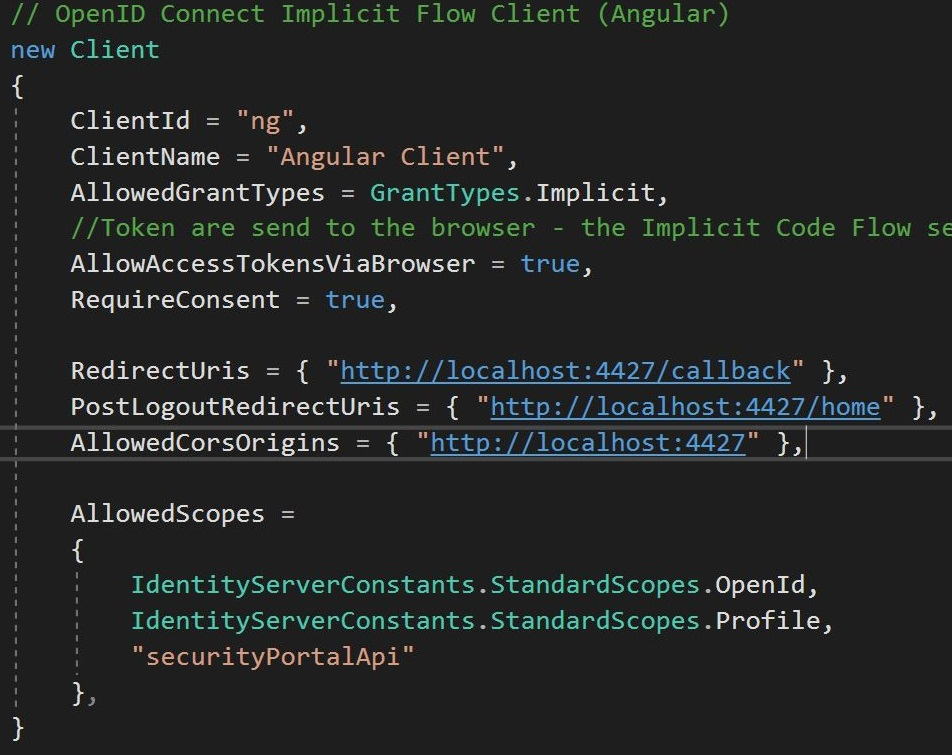
\includegraphics[width=0.8\linewidth]{images/implicit_code_flow}
	\caption{Implicit Code Flow - Identity Server Configuration}
	\label{fig:implicitcodeflow}
\end{figure}


AllowAccessTokensViaBrowser makes sure that the access\_token can be directly returned to the browser after the client authenticates itself. AllowCorsOrignins allows the given resource to make Cross-Origin-Requests to the Identity Server. Cross-Origin-Request is a request that is made from another domain outside the domain from which the first resource was served. Furthermore, the RedirectUris have to be present, in order for the Identity Server to know where to return after the login attempt was successful. 


In the Angular Solution, a service to handle authentication was created. The service handles requests to the API which is hosting the protected resources. The Angular Solution uses the ‘oidc-client’ library that is suggested by the Identity Server framework to handle authentication requests. To call the Identity Server the following setting are used, shown in figure~ \ref{fig:implicitcodeflowangular}.

\begin{figure}[h]
	\centering
	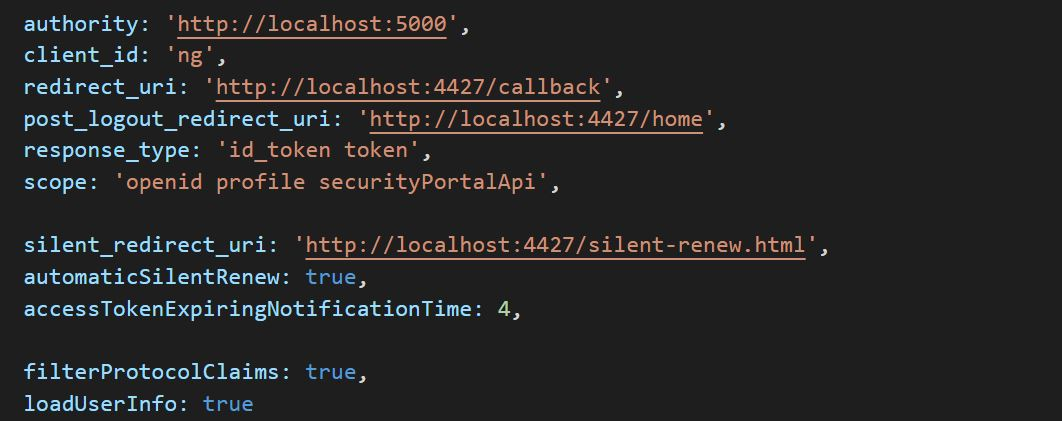
\includegraphics[width=0.8\linewidth]{images/implicit_code_flow_angular}
	\caption{Implicit Code Flow - Angular}
	\label{fig:implicitcodeflowangular}
\end{figure}


The client\_id in the Angular Solution has to be the same as the ClientId configured in the Identity Server Project. The same is true for the redirect\_uri and post\_logout\_redirect\_uri. Otherwise, the request would result in an error. For example, if a scope is requested which does not exist accordingly to the Identity Server, an invalid scope exception is thrown. Furthermore, the response\_type has to be according to the used Authorization Flow in the in IdentityServer's client configuration. In the Identity Server Solution, the  Implicit Code Flow was configured, therefore "id\_token token" was defined. The response of these response types will include an access token, an access token type and an id\_token.  

\begin{figure}[h]
	\centering
	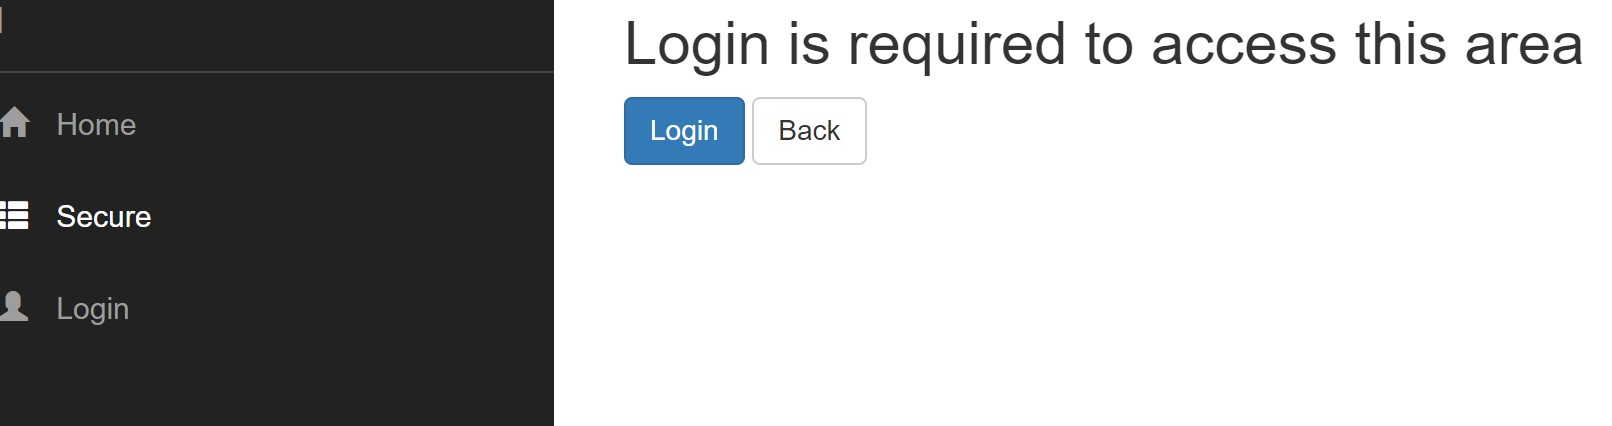
\includegraphics[width=0.8\linewidth]{images/secure_page_requires_login}
	\caption{Secure Page Login}
	\label{fig:securepagerequireslogin}
\end{figure}

For the Client to receive an id\_token and in this example an access\_token from the Authorization Server (Identity Server Project), the client has to prepare an Authentication Request and send it to the Authorization Server. The Angular Client has two possible ways to trigger the login with the Identity Server. In the navigation on the left-hand side there is a Home Page that can be accessed by everyone, then there is a Secure Page that just can be accessed by logged in users and the Login Page, which automatically triggers a request to the Authorization Server.



The figure~\ref{fig:securepagerequireslogin}, shows the Menu of the application. If the user tries to access the Secure Page without being logged in he is redirected to the "Login is required" Page. In order to access the secure area, the End-User has to authenticate with the Authorization Server.
To authenticate with the Authorization Server the user has to press the Login button. After the Login button is pressed, the End-User is redirected to the Authorization Server Login Page. The design of this screen can be adjusted in the Identity Server Project. 

\begin{figure}[h]
	\centering
	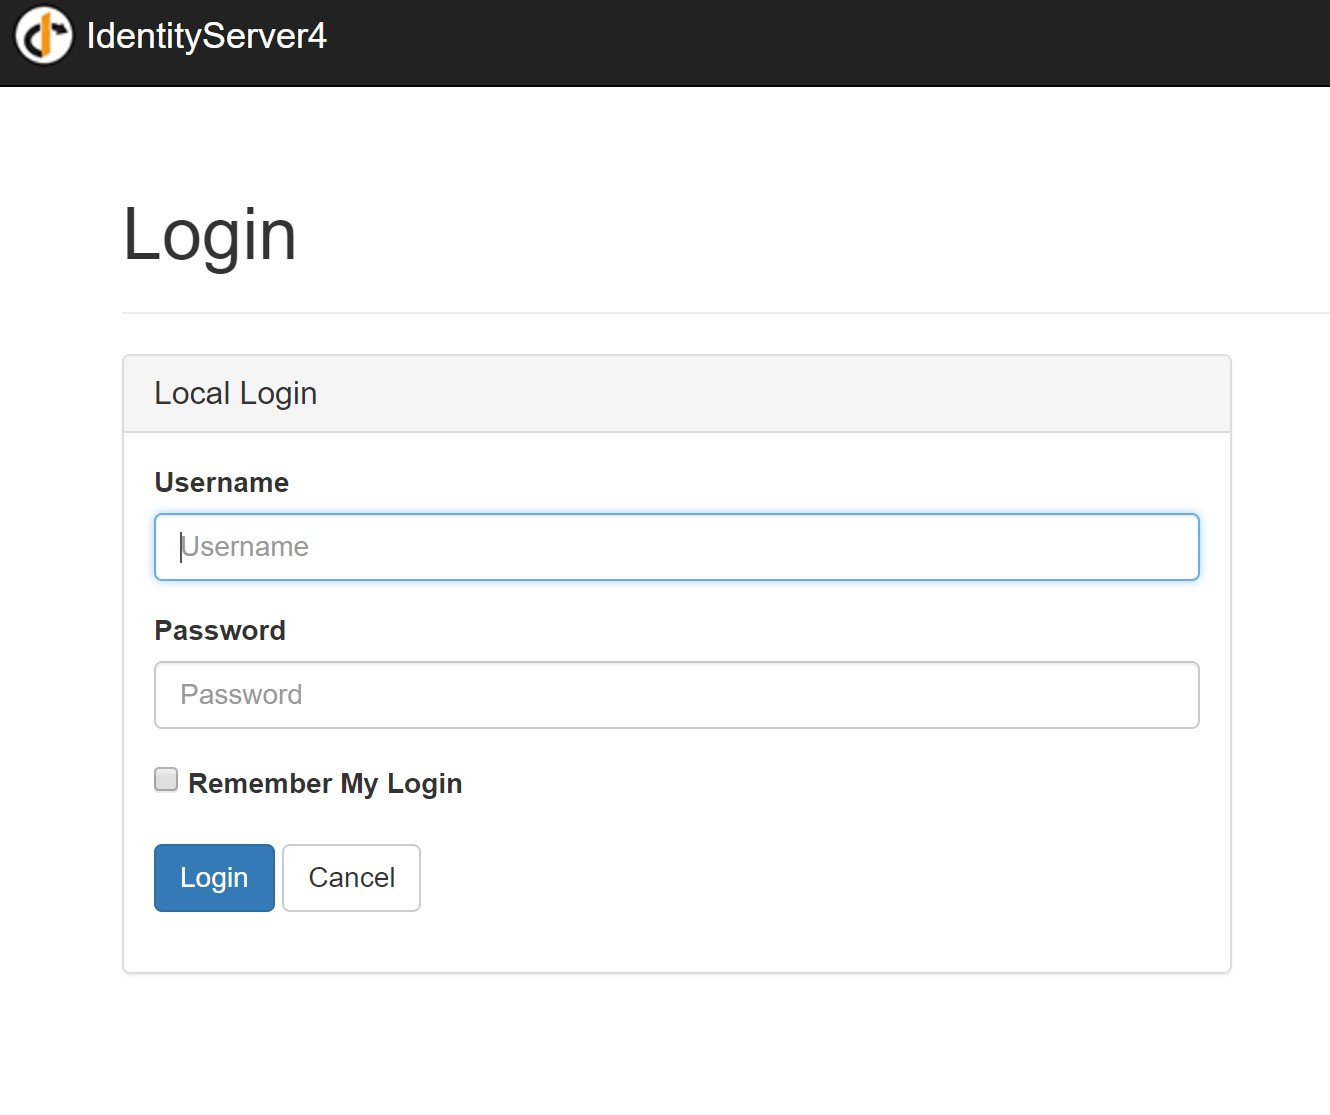
\includegraphics[width=0.7\linewidth]{images/login_identity_server}
	\caption{Login Mask Identity Server}
	\label{fig:loginidentityserver}
\end{figure}


The (figure~\ref{fig:loginidentityserver}), shows the form where the end-user can log in with the end-user’s credentials. In the Identity Server Project, two test-user are registered. Therefore either Alice or Bob can currently log in to the application and view the secured Page. 
The Authorization Server can also request consent from the User for the requested Claims. In the Identity Server Project, it is configured that the consent of the End-User is required. In consequence of this configuration, the user is prompted an additional screen. This screen is shown in figure~ \ref{fig:consentscreen}, it would not appear if the consent was not required by the identity server. 

\begin{figure}[h]
	\centering
	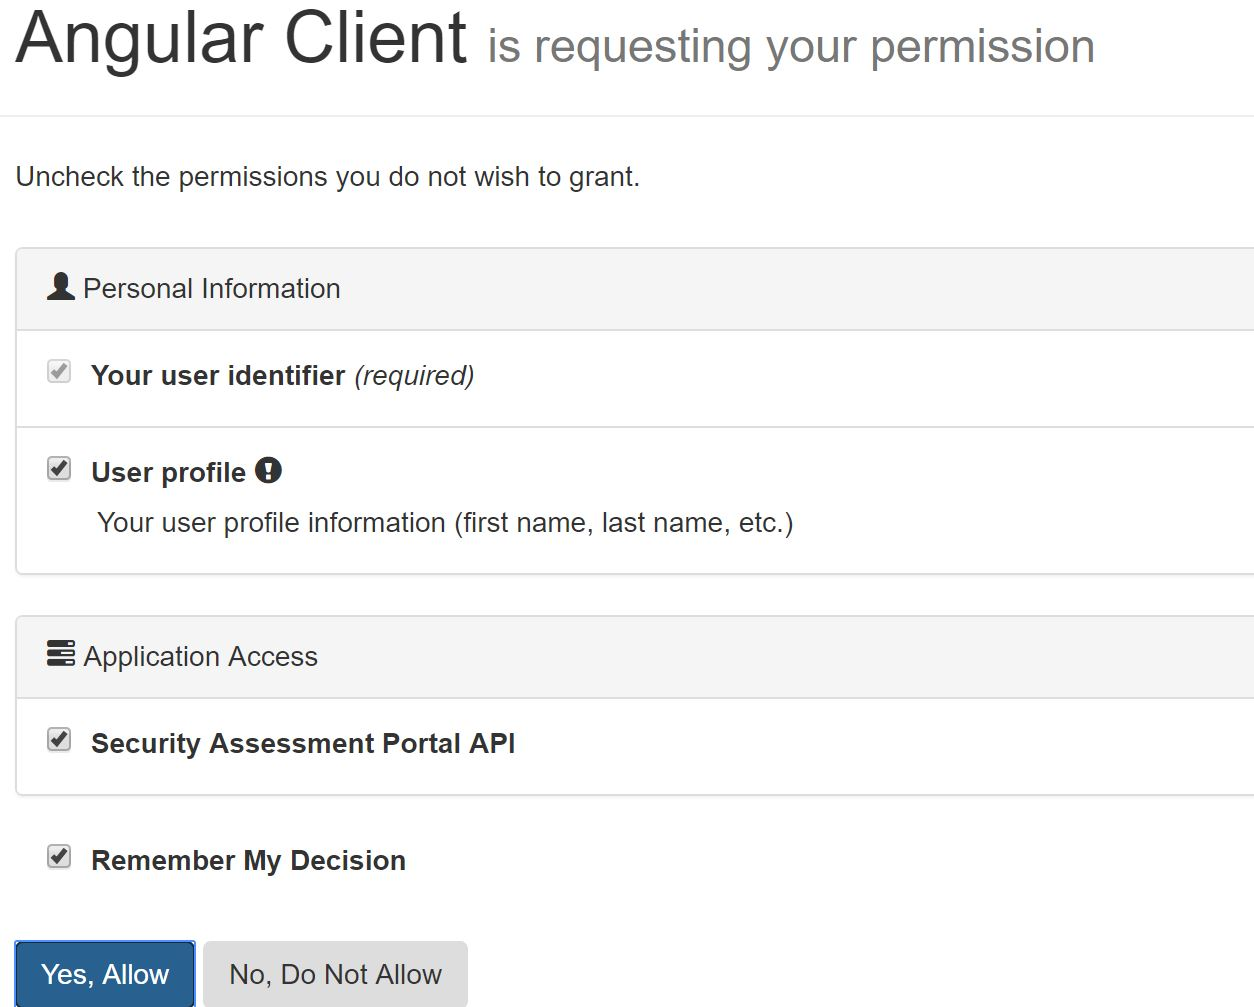
\includegraphics[width=0.7\linewidth]{images/consent_screen}
	\caption{Consent Screen}
	\label{fig:consentscreen}
\end{figure}


The Angular Application is requesting consent for the requested scopes openId, profile and securityPortalApi. The openId Scope is required because otherwise, we would not be able to receive an id\_token. User Profile gives additional information about the User, and the  Security Assessment Portal API is a custom API that was added to the scope and allows the user to make requests to this API and the protected resources. 


After the End-User has given its consent, the End-User gets redirected back to the Client with an id\_token and an access\_token. The id\_token can be validated and an End-User’s Subject Identifier is retrieved.

If the authentication with the Authorization Server was successful the End-User is now authenticated. As an authenticated user the End-User can now also access the Secure Page. With access\_token the received access token calls to the custom API Project can be executed. For example, the claims of the user that are correlating to the scopes can be received and put in a useful context as seen in figure~\ref{fig:claims}.


\begin{figure}[h]
	\centering
	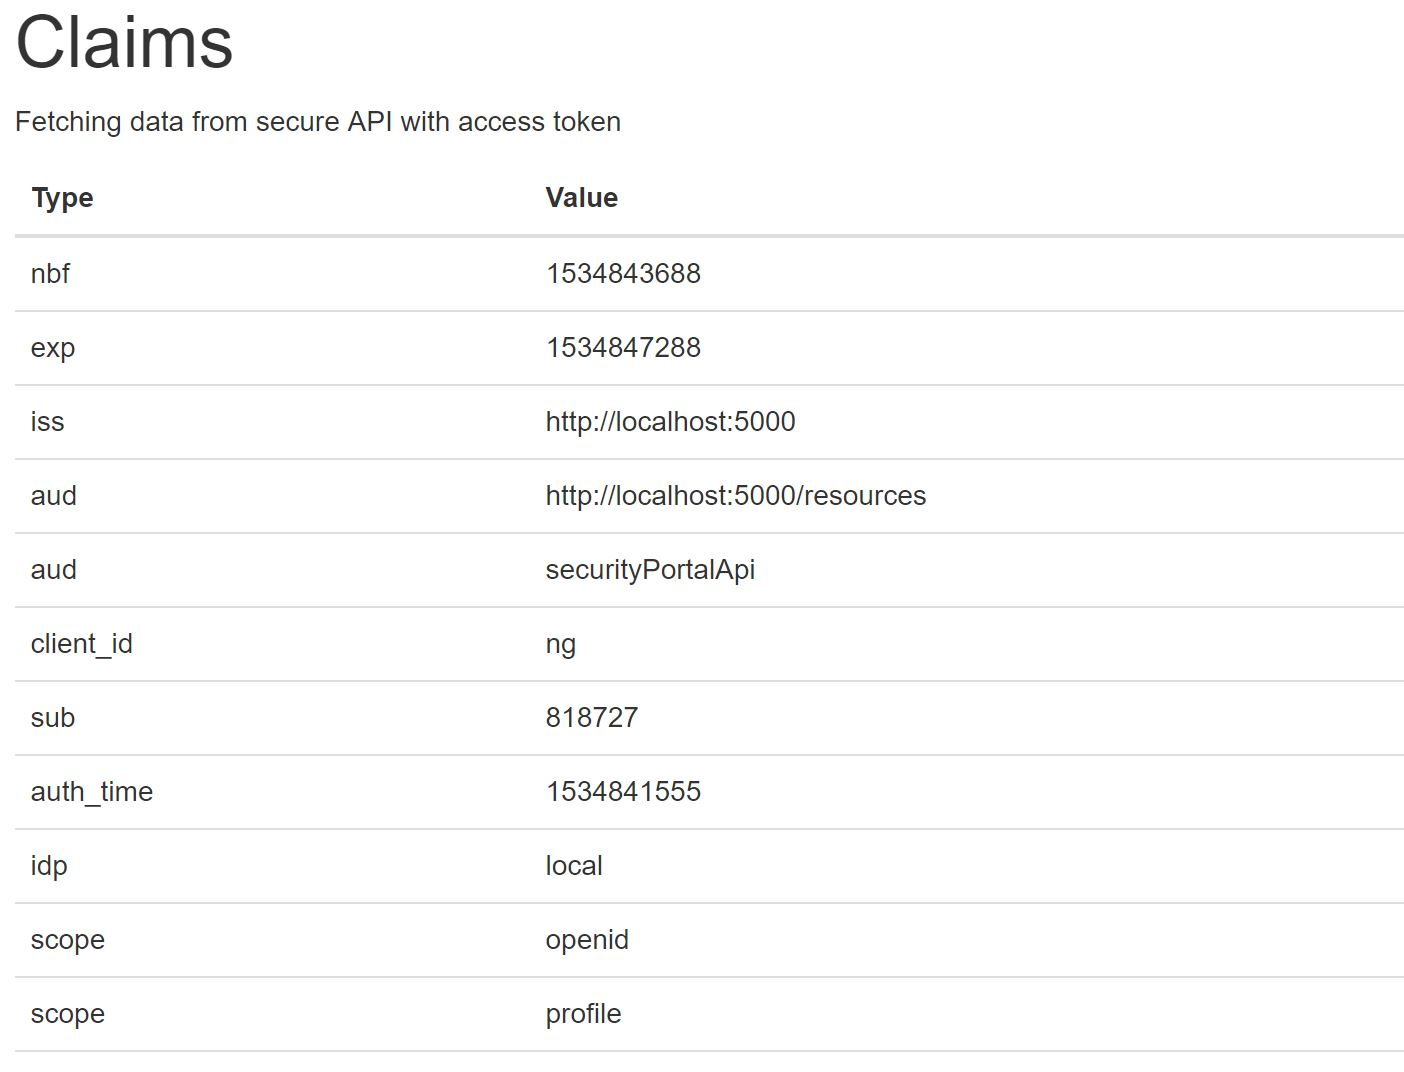
\includegraphics[width=0.7\linewidth]{images/claims}
	\caption{Claims}
	\label{fig:claims}
\end{figure}


This complete example could be a possible implementation of the authentication for the described use case in section \ref{usecase}. Now it would also be possible for an external user (customers) to access the application without a domain account. If customers also choose to use other products of the companies, no new account is required because the same identity server can be used. The personal data of the customers stays in the company and is not given to any third party. With the use of token-based authentication, it is easy to manage the session of end-users, and the user can stay logged in the application (single-sign-on). The use of bear tokens gives appropriate security and the implicit flow used to deliver the token makes it very light-weighted for single page application. The separated API is also convenient because it might be used for multiple purposes.

\chapterend
